\documentclass[11pt, a4paper]{article}
\usepackage[utf8x]{inputenc}
\usepackage[swedish, english]{babel}		% last is active
\usepackage{graphicx}
\usepackage{amsmath}					% to be able to \split eqs
\usepackage{amssymb}					% Real/Imaginary fonts
\usepackage{units}
\usepackage[tight, hang]{subfigure}
\usepackage{url}
\usepackage{tikz}						% for drawing
\usetikzlibrary{shapes, arrows, decorations.markings, decorations.pathmorphing, decorations.pathreplacing, calc}
\usepackage{fancyhdr}
\usepackage{float}						% H-positioned and custom floats
\usepackage{datetime}					% to fix date format
\usepackage[usenames,dvipsnames]{pstricks}
%\usepackage{epsfig}
%\usepackage{pst-grad} % For gradients
%\usepackage{pst-plot} % For axes
\usepackage{pgfplots}
% =================== some local stuff ================= %
\newcommand{\degree}{\ensuremath{^\circ}}
\newcommand{\todayswe}{\the\year-\twodigit\month-\twodigit\day}


\def\contacts{Torbjørn Ludvigsen, tolu0022@student.umu.se\\Olof Lenti, olle0004@student.umu.se\\
Yunus Gures, yunusgures@gmail.com}
\def\names{Torbjørn Ludvigsen, Olof Lenti, Yunus Gures}
\def\dept{Department of Physics}
\def\course{Non invasive measurement theory}
\def\lab{Optical measurements:\\Determination of the Damping of a Pendulum with Time of Flight}
\def\supervisors{Patrick Ehlers\\Isak Silander\\ Amir Khodabakhsh}
\date{\todayswe}
% custom commands
\newcommand\OpVec[1]{\boldsymbol{\hat{#1}}}		% bold with hat for operator vectors
%\newcommand\Sup[1]{\textsuperscript{\tiny{#1}}}		% 1st, 2nd.. and so on
\newenvironment{eqn}{\begin{equation*} \begin{split}}{\end{equation*} \end{split}}
% header

% document
\begin{document}
\pagestyle{fancy}
\begin{titlepage}
	\begin{center}
		\course\\
		\Large{\lab}\vspace{2mm}
		\hrule\vspace{2mm}
		\tiny{\contacts}\vspace{2mm}
		\hrule
	\end{center}
	\vspace{4mm}

	\begin{abstract}

  $\alpha_{alu} =\unit[(23.0 \pm 0.1)\cdot10^{-6}]{K^{-1}}$ 

  $\alpha_{sst} = \unit[(15.8 \pm 0.2)\cdot10^{-6}]{K^{-1}}$, 
    which is only 1 \% off tabulated values \cite{ph, thex}.

	\end{abstract}
	\vfill
	\hrule\vspace{2mm}
	\centering
		\tiny{Supervisor: \supervisors}
	%\end{center}
\end{titlepage}

\pagestyle{plain}
\vspace{2cm}
\section{Introduction}

\section{Theory}
\subsection{Optics}
\subsection{Circuits}
\subsection{maths}

blabla
The forces considering air drag are described differently for different velocities. For very low velocities i.e. when the pendulum is at its turning point the drag force will be proportional to the velocity as

\[
F_d = -bv,
\]
where $F_d$ is force of drag, $v$ is the velocity and $b$ is a positive constant.
For higher velocities the force of 

\begin{figure}[H]
	\centering
	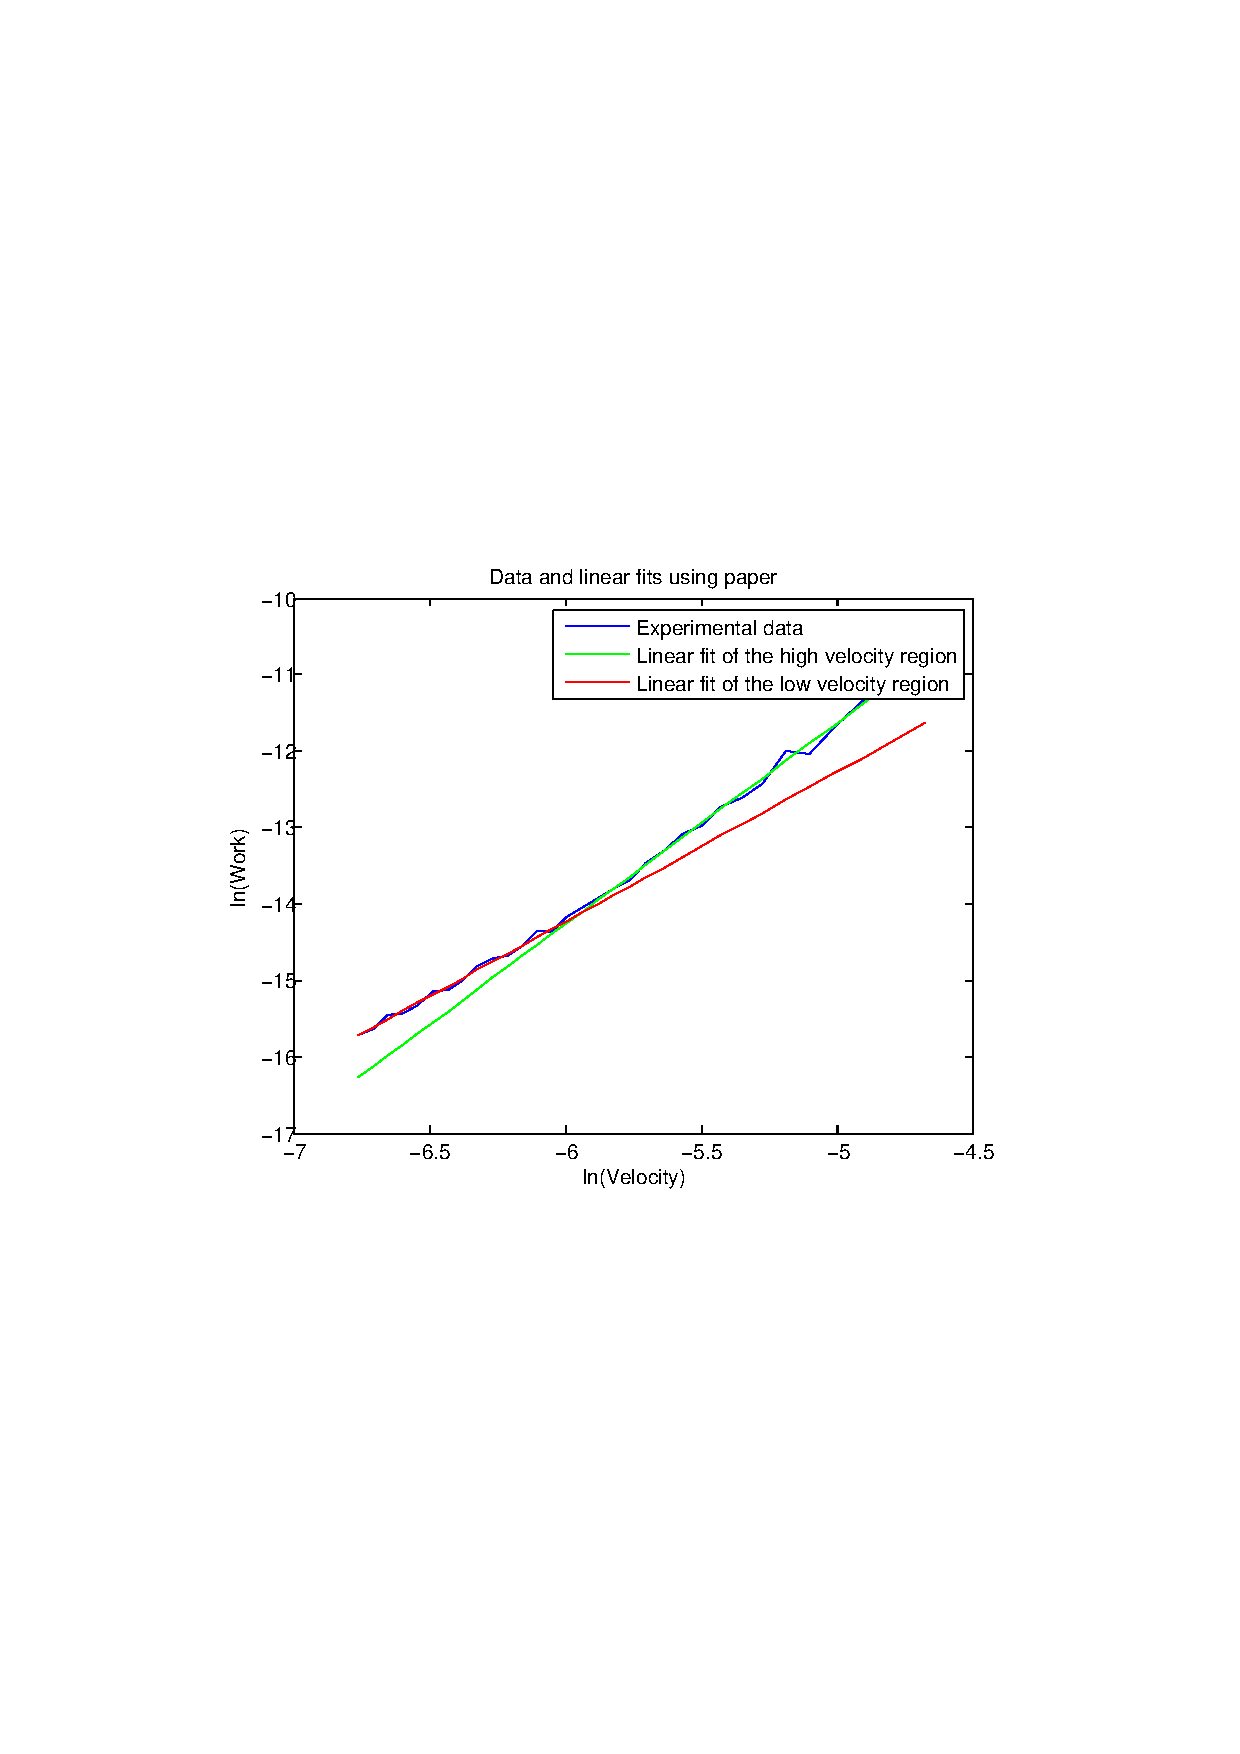
\includegraphics{paper}
	\caption{Helmholtz resonator}
	\label{f:helmholtz}
\end{figure}



By beginning with the equation
\[
v_{max} = Ce^{at} + De^{bt}.
\]
By breaking out $e^{at}$ and taking the logarithm we end up with the equation
\[
\ln(v_{max}) = \ln(C + De^{\frac{b}{a}t}) + at
\]
For small $t$ the first term will be nearly constant. A linear fit can be made to find the slope $a$.
In a similar fashion we can break out $e^{bt}$

\section{Experimental Setup}
\section{Procedure}
\section{Error calculations}
\section{Results}
\section{Discussion}
\section{Summary and Conclusions}
\vfill

\begin{thebibliography}{99}
	\bibitem{ph} Nordling, C., Österman, J. (2006). 
  \textit{Physics Handbook  $8^{th}$}\\
  Lund, Sweden, Studentlitteratur.
\end{thebibliography}

\begin{appendix}
\end{appendix}

% nY KOMMENTAR

\end{document}
%\begin{figure}[H]
%	\centering
%	\begin{tikzpicture}[scale = 0.95]
%		\def\mr{1.5};
%		\draw (0,0) ellipse (0.5 and \mr);
%		\begin{scope}
%			\clip (0,0) ellipse (0.5 and \mr);
%			\foreach \i in {0, 1, ..., 15} {
%				\draw (-0.5, {-3 + 0.25*\i}) -- (0.5, {-1 + 0.25 * \i});
%			}
%		\end{scope}
%		\path[fill = white, opacity = 0.7] (0, 0) circle (0.2);
%		\node at (0, 0) {$S$};
%		\begin{scope}
%			% overlapping regions will cancel out
%			\draw[fill = white] (5, 0) circle (3);
%		\end{scope}
%		\draw (0, \mr) -- ++(2.8, 0) to[out = 0, in = -135] ++(0.3, 0.3)
%			  (0, -\mr) -- ++(2.8, 0) to[out = 0, in = 135] ++(0.3, -0.3);
%		\node at (5, 0) {$V$};
%	\end{tikzpicture}
%	\caption{Helmholtz resonator}
%	\label{f:helmholtz}
%\end{figure}
